\newgeometry{margin=85pt}
\chapter*{Sistemas de Información Geográfica}
\setcounter{chapter}{2} 
\setcounter{section}{0}
\addcontentsline{toc}{chapter}{Sistemas de Información Geográfica}

Un Sistema de Información Geográfica (SIG) o \textit{Geographical Information System} (GIS), es un entorno para capturar, almacenar, gestionar y analizar datos geográficos.
Lo cierto es que la definición de GIS es mucho más compleja que la anterior, además existen infinidad de definiciones sobre el término GIS, 
según la ciencia en la que se encuentre enmarcado o según funcionalidades, arquitectura, aplicaciones u objetivos que persigue. 
No vamos a entrar en los distintos puntos de vista que encontramos en la literatura sobre los GIS, pero sí que resulta interesante destacar la definición propuesta por
el National Center for Geographic Information and Analysis (NCGIA): “Un SIG es un sistema de información compuesto por hardware, software y procedimientos para capturar,
manejar, manipular, analizar, modelizar y representar datos georeferenciados, con el objetivo de resolver problemas de gestión y planificación”.

Antes de profundizar en cada parte de los GIS que aparece en la definición, vamos a definir lo que se entiende por Información Geográfica y las propiedades que presenta.

\section{Información Geográfica} \label{sec:geoinfo}
La información geográfica se define como “cualquier dato espacial, que de forma directa o indirecta, hace referencia a una localización o zona geográfica específica”,
tal y como se establece en el artículo 3.2 de la Directiva INSPIRE \cite{directiva-INSPIRE}. 
En este sentido, podemos entender como información geográfica todos aquellos datos que hacen referencia a descripciones espaciales.

Según el Glosario multilingüe de ISO/TC 211, los términos “datos espaciales” y “datos geográficos” son sinónimos, y
se definen como los datos que implícita o explícitamente se refieren a una localización relativa a La Tierra.

Por tanto, se pueden considerar como datos geográficos una dirección, un código postal o un punto definido mediante un sistema de coordenadas geográficas, entre otros.

Los datos geográficos presentan dos tipos de propiedades fundamentales: geométricas y descriptivas.

\subsection{Propiedades geométricas}

Las propiedades geométricas son aquellas que están vinculadas con la referencia espacial, conocida como “georeferenciación”.
La georeferencia de un dato geográfico se define mediante su posición, la cual puede ser absoluta, sobre un sistema de coordenadas (\textit{x}, \textit{y}, \textit{z}), 
o relativa, respecto a otros elementos del paisaje, con los que define relaciones topológicas. 
“La topología expresa las relaciones entre los objetos de forma cualitativa: si dos polígonos son colindantes (contigüidad), si uno
está contenido en el otro (inclusión), si dos líneas están conectadas (conectividad)” \cite{Puebla-Gould}.

Las posiciones pueden agruparse para localizar una región del espacio, a través de distintas figuras geométricas:
\begin{itemize}
  \item Puntos: Los puntos representan objetos cuya dimensión es insignificante o nula para una determinada área. 
  Por ejemplo, casas, torres de vigilancia, estaciones pluvimétricas. Los datos que refieren a objetos con dimensión de área escasa
  pero considerable extensión vertical también son tratados como puntos. Es el caso de los pozos de las perforaciones geológicas
  o mediciones subterráneas que aportan datos sísmicos.
  \item Líneas: Las líneas representan objetos cuya dimensión espacial es la longitud. Se definen mediante listas de pares de coordenadas (\textit{x}, \textit{y}) y pueden representar
  ríos, caminos, líneas del tendido eléctrico, etc.
  \item Áreas: Las superficies representan objetos que existen como superficies o áreas que pueden representarse como polígonos definidos cómo una serie
  cerrada de puntos de coordenadas espaciales. Por ejemplo, los municipios y los espacios naturales se representan mediante superficies.
  \item Volúmenes: Los volúmenes representan objetos tridimensionales, como por ejemplo son el relieve o las edificaciones.
\end{itemize}

\begin{figure}[H]
  \centering
  \subfigure[Puntos - Centros sanitarios]{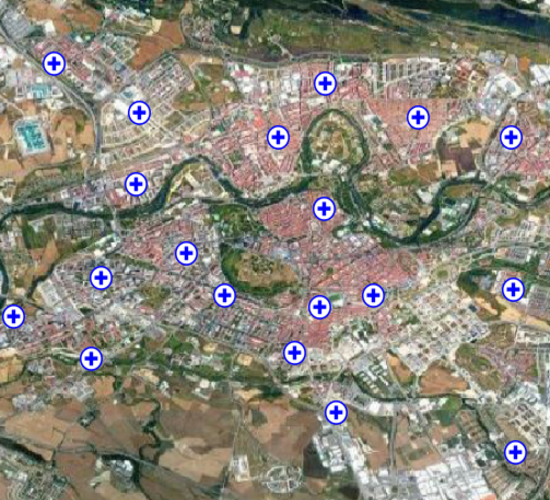
\includegraphics[width=0.35\columnwidth]{Imagenes/GIS/centros-sanitarios.png}}
  \subfigure[Líneas - Red hidrográfica]{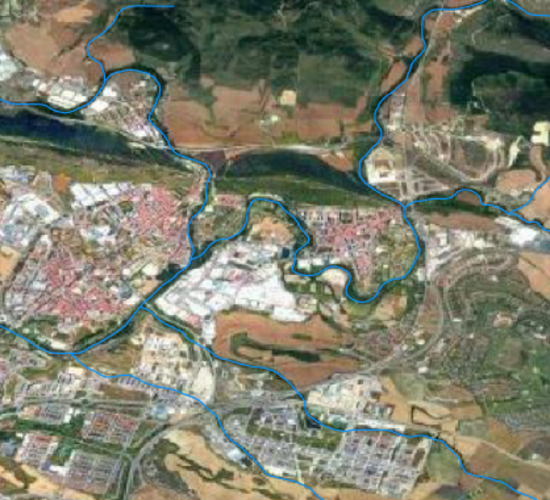
\includegraphics[width=0.35\columnwidth]{Imagenes/GIS/rios.png}}
  \subfigure[Áreas - Núcleos de población]{\includegraphics[width=0.35\columnwidth]{Imagenes/GIS/nucleos-población.png}}
  \subfigure[Volúmenes - Edificaciones]{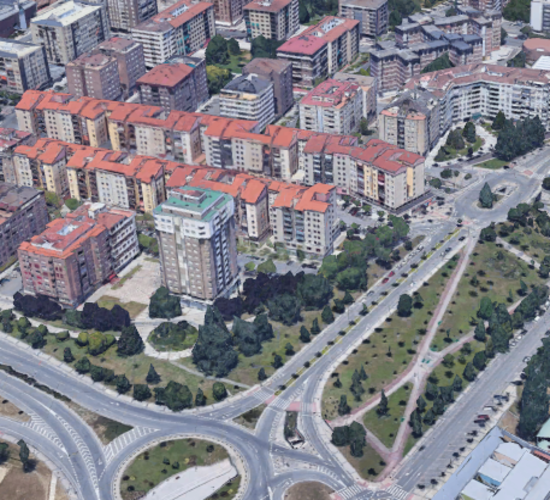
\includegraphics[width=0.35\columnwidth]{Imagenes/GIS/edificios3D.png}}  
  \caption{Representaciones de datos geográficos a través de figuras geométricas} \label{fig:dimensiones} 
\end{figure} 

La figura \ref{fig:dimensiones} muestra ejemplos concretos de representaciones geográficas visualizadas sobre el mapa.

\subsection{Propiedades descriptivas}

Además de las propiedades geométricas, la información geográfica está compuesta por propiedades descriptivas.
Estas propiedades constan de información cuantitativa/cualitativa que aporta un valor diferenciado entre los datos.
Esta información se define en forma de atributos, que pueden ser puede ser discretos o continuos.

\begin{itemize}
  \item Atributos discretos: el conjunto de valores que puede tomar el atributo asociado al espacio geográfico es discreto,
  como por ejemplo el tipo de cultivo o la capacidad de un canal.
  \item Atributos continuos: el valor asociado a los puntos del espacio puede variar de modo gradual a lo largo del espacio geográfico,
  como por ejemplo la salinidad del suelo, la temperatura o la presión atmosférica.
\end{itemize}

En definitiva, los objetivos que persiguen los GIS son el reconocimiento de las relaciones topológicas y geométricas que existen entre los elementos geográficos, 
y el manejo de las características temáticas (atributos).

\section{Componentes}

\begin{figure}[H]
  \centering
  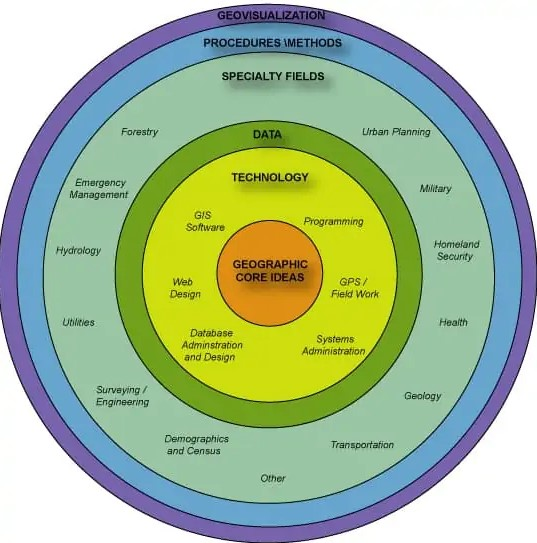
\includegraphics[width=0.45\textwidth]{Imagenes/GIS/Componentes-GIS.jpg}
  \caption{Componentes GIS} \label{fig:compnentesGIS}
\end{figure}

Los GIS han evolucionado a lo largo del tiempo, de modo que la interpretación del concepto ha ido aumentando en dimensión y complejidad. 
Por ello, es importante clasificar sus componentes según su importancia. En \cite{components-GIS}, se proponen 6 componentes de los GIS, 
los cuales podemos observar en la figura \ref{fig:compnentesGIS} en forma de anillos concéntricos.

\begin{itemize}
  \item Geographic Core Ideas\\
  El núcleo de los GIS es la teoría en la que están basados estos sistemas, como por ejemplo la geografía, topología, geodesia, etc. 
  A partir de estos conocimientos, surgen problemáticas o planteamientos geográficos que se quieren resolver a partir del análisis de la información geográfica.

  \item Tecnología\\
  El anillo que envuelve el core de los GIS, corresponde a todas las necesidades tecnológicas que estos requieren. 
  Agrupa tanto software como hardware, incluyéndose tareas administrativas para la gestión de los GIS y de los Sistemas Gestores de Bases de Datos que nutren de datos a los GIS.
  En la sección \ref{sec:herramientas}, veremos algunos de los productos GIS más populares.

  \item Datos\\
  En este componente se incluye cualquier información geográfica, detallada en la sección \ref{sec:geoinfo}.
  Más adelante, en la sección \ref{sec:datos}, veremos la forma en la que los GIS gestionan los datos.
  En estos últimos años, el manejo de los datos ha cobrado más importancia que el software propio de GIS, debido al gran volumen de datos que se generan. 
  Existe un exceso de datos provenientes, entre otros, de los dispositivos IoT, que recopilan datos constantemente. 
  La mayoría de esta información esta georeferenciada, pero no está estructurada.   
  Por otro lado, exiten sistemas de observación terrestre, como sensores, satélites o vuelos digitales. 
  Esta información si se encuentra estructurada, ya que es capturada y documentada por distintos organismos e instituciones (en la sección \ref{sec:datos} comentaremos algunas de ellas).
\\
  \item Especialidades\\
  En el componente de Especialidades, se incluyen todos aquellos campos de la geografía o que hacen uso de ella para resolver cuestiones relacionadas con una profesión o sector.
 
  \begin{figure}[H]
    \centering
    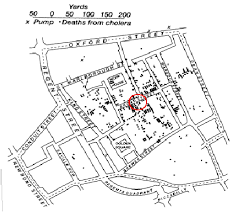
\includegraphics[width=0.30\textwidth]{Imagenes/GIS/Snow-cholera-map.png}
    \caption{Mapa de Snow en su estudio sobre cólera} \label{fig:SnowColeraMap}
  \end{figure}

  Uno de los campos que aparece en la figura \ref{fig:SnowColeraMap}, es el campo de la salud, en el que se incluye el trabajo de de Dr. John Snow. de 1854, 
  con el que consiguió identificar el origen de un brote de cólera en Londres, el cual se encontraba en una de las fuentes de la ciudad.
  Para ello, creó el mapa de la figura, a partir de datos de estudio, en el que se observa un patrón claro que nadie había observado todavía.  
  
  \item Procedimientos/Métodos\\
  Este componente está referido a las distintas formas de trabajo de cada campo del componente anterior. 
  Los equipos que trabajen con GIS, deben planificar el uso de los datos espaciales, la tecnología que mejor se ajuste a ellos y la forma de presentar los resultados al usuario final.

  \item Geovisualización\\
  Resulta verdaderamente importante la presentación de datos al usuario final, ya que nos va a permitir que el análisis de los datos nos sirva en la toma de decisiones.
  Esta representación del espacio y el tiempo puede tomar la forma de mapas, gráficos, diagramas, animaciones y simulaciones.
\end{itemize}

\section{Funciones}
La potencia de un GIS está en las utilidades o análisis que se pueden realizar con la información. Las más básicas pueden ser:

\begin{itemize}
\item Captura \\
El proceso de captura de la información geográfica se basa en la digitalización de los datos, es decir, pasar los datos a una forma analítica. 
Hay muchas formas diferentes de recopilar datos GIS. Por ejemplo, a través de sistemas LiDAR , drones , GPS o satélites.
\item Almacenamiento \\
En la mayoría de casos se realiza un preprocesamiento de los datos capturados para su correcta estructuración.
\item Consulta \\
La información capturada y almacenada debe poder ser gestionada por el GIS, permitiendo realizar búsquedas temáticas, espaciales y con capacidad de
selección multicondicionadas para su posterior análisis.
\item Análisis \\
Uso de métodos espaciales y estadísticos para analizar tanto las propiedades geométricas como las descriptivas de la información geográfica
(dichos métodos se explicarán más detalladamente en el capítulo \ref{cap:analisis}).\\
Esta función es la específica de los GIS y es su elemento característico. 
\item Visualización de resultados \\
Presentación de los datos es en su proyección sobre el espacio bidimensional o tridimensional, definido mediante coordenadas cartesianas.
\end{itemize}

\section{Datos espaciales} \label{sec:datos}

\subsection{Representación digital} 
Los datos geográficos se representan en forma de capas de información.
En los GIS, las capas definen los distintos formatos con los que se representan los datos geográficos, en concreto,
especifican qué características siguen y con qué forma se estructuran.

En función de la tipología de los datos, podemos identificar dos tipos de capas:
\begin{itemize}
  \item Capa ráster\\
  Los datos están dispuestos en una malla rectangular de celdas, cuadrados o píxeles.
  Cada píxel dentro de un ráster tiene un valor, como color, altura, temperatura, velocidad del viento u otras medidas.
  Algunos ejemplos de capas ráster lo vemos en las imágenes satélite, en dónde cada pixel tiene un color asociado, 
  o en los mapas de elevación, dónde cada pixel está representado por una altura específica.

  \begin{figure}[H]
    \centering
    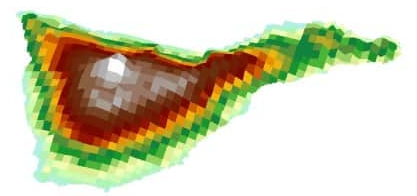
\includegraphics[width=0.50\textwidth]{Imagenes/GIS/mapa-elevacion.png}
    \caption{Modelo Digital de Elevación} \label{fig:mapaElev}
  \end{figure}

  En la figura \ref{fig:mapaElev} podemos observar un modelo digital de elevación en dónde los pixeles se componen de un color en base a la altitud del terreno.

  \item Capa vectorial\\
  Las capas vectoriales, como su propio nombre indica, están formadas por datos vectoriales, los cuales representan geometrías en el espacio.

  \begin{figure}[H]
    \centering
    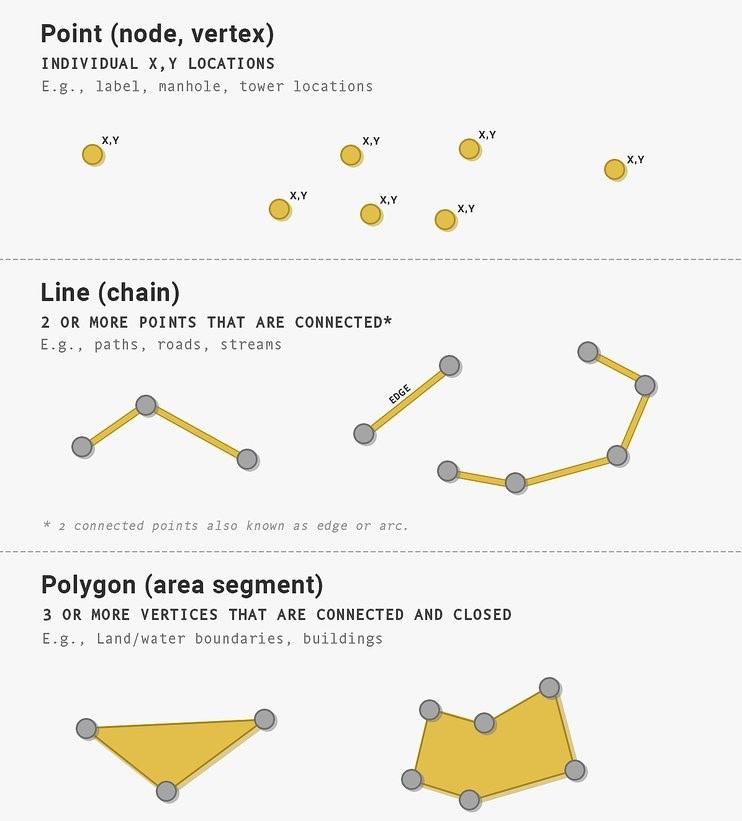
\includegraphics[width=0.7\textwidth]{Imagenes/GIS/geometrias-capa-vectorial.jpg}
    \caption{Tipos de vectores} \label{fig:geoVectorial}
  \end{figure}

  Tal y como se muestra en la figura \ref{fig:geoVectorial}, las tres geometrías principales son los puntos, las líneas y los polígonos (líneas conectadas que encierran un área en su interior).
  Podemos usar vectores para presentar características y propiedades en la superficie de La Tierra.
  Como por ejemplo, asociando la dirección como atributo de los centros sanitarios, mostrados en la figura \ref{fig:dimensiones}(a), los cuales se representan mediante puntos.
\end{itemize}

\begin{figure}[H]
  \centering
  \subfigure[Capa ráster]{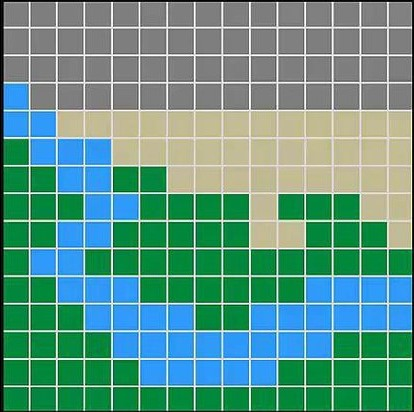
\includegraphics[width=0.35\columnwidth]{Imagenes/GIS/capa-raster.jpg}}
  \subfigure[Capa vectorial]{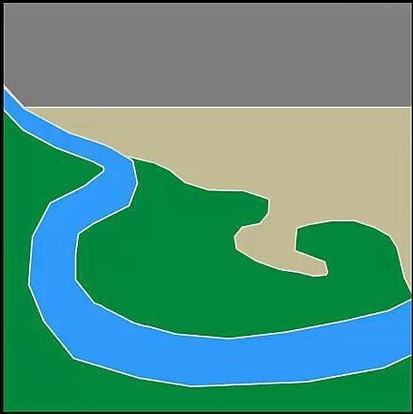
\includegraphics[width=0.35\columnwidth]{Imagenes/GIS/capa-vectorial.jpg}}
  \caption{Representación de los datos geográficos} \label{fig:capas} 
\end{figure} 

Como hemos visto en los puntos anteriores, la diferencia principal entre las capas, es la forma en la que representan los datos geográficos, cuya diferencia queda expuesta en el ejemplo de la figura \ref{fig:capas}.

Cada representación de los datos geográficos tienen sus ventajas e inconvenientes, por ejemplo,
las capas ráster son adecuadas para modelar aspectos del medio muy variables, en cambio, 
las capas vectoriales son más adecuadas para modelizar aspectos poco variables, generalmente cualitativos.
Por otro lado, las capas vectoriales permiten definir los límites entre distintos objetos de forma más precisa, en  cambio, 
las capas ráster presentan límites basados en el propio tamaño de píxel y tienen ciertas dificultades para desarrollar análisis espaciales.

\subsection{Gestión en los GIS}

El GIS incorpora un gestor de capas que permite al usuario ordenar, añadir y eliminar capas, de forma que permite construir mapas dinámicos. 
Además, permite al usuario almacenar de forma permanente configuraciones interesantes que pueden ser recuperadas más adelante.
También permite realizar análisis más profundos y complejos que con otros sistemas.
Por ello, podemos representar situaciones reales o escenarios simulados de gran utilidad, como por ejemplo, para analizar la distribución y el índice de pobreza de un país a lo largo del tiempo.

El camino que nos permite modelar problemáticas que tenemos en la realidad a través de los GIS, pasa por la construcción de los siguientes modelos:
\begin{itemize}
  \item Modelo geográfico\\
  El modelo geográfico es el modelo conceptual de la realidad geográfica, es decir, el fenómeno del que partimos. 
  En el ejemplo de la pobreza de un determinado país, necesitamos representar un modelo conceptual en el que, por ejemplo, las ciudades pueden ser las unidades conceptuales objeto de estudio.
  Cada una de ellas con una serie de propiedades descriptivas, y que se relacionan geográficamente entre sí por sus propiedades geométricas, cuya representación tenemos que modelar.  
  \item Modelo de representación\\
  El modelo de representación es la forma de reducir a un conjunto finito de elementos el modelo geográfico definido anteriormente. 
  Por ejemplo, una vez definido a las ciudades como objeto de estudio, podemos representarlas como puntos en el espacio total, en este caso el territorio de un país.
  La distancia entre puntos puede representar la distancia real que existe entre las ciudades o/y el tamaño de los puntos puede ser proporcional al número de habitantes que vivan es esa cuidad.
  En otros estudios nos puede interesar representar las ciudades como polígonos, por ejemplo para hacer explícita la superficie de esa ciudad.
  \item Modelo de almacenamiento\\
  El modelo de almacenamiento es un esquema que define la forma de guardar los distintos elementos del modelo de representación. 
  Por ejemplo, podemos almacenar las ciudades como imágenes comprimidas y sus características almacenadas en una hoja de Excel.
\end{itemize}

\subsection{Fuentes} \label{sec:fuentes}

Antes de entrar en los distintos servicios que permiten la captura de información geográfica, es necesario conocer la legislación vigente a nivel europeo para la exposición de este tipo de información.
La Infraestructura de Información Espacial en Europa o \textit{Infrastructure for Spatial Information in Europe} (INSPIRE), 
ha sido desarrollada por la Comisión Europea con el propósito de hacer disponible información geográfica relevante, concertada y de calidad,
de forma que se permita la formulación, implementación, monitorización y evaluación de las políticas de impacto o de dimensión territorial.
Dicho funcionamiento se recoge en la Directiva \cite{directiva-INSPIRE} del Parlamento Europeo.
Algunos de los servicios que en ella se especifican, están basado en estándares \textit{Open Geospatial Consortium} (OGC) \cite{OGC}.
El OGC es un consorcio internacional formado por más de 500 entidades, entre las cuales se encuentran empresas, agencias gubernamentales, centros de investigación y universidades, 
con el objetivo de exponer servicios de información geoespacial de forma fiable, accesible, interoperable y reutilizable.

Por lo tanto, las fuentes de datos espaciales comentadas a continuación deben responder a los requisitos definidos por la Directiva \cite{directiva-INSPIRE}. 

A nivel nacional, algunos Ministerios facilitan el acceso a los datos espaciales que generan.
\begin{itemize}
  \item El Instituto Geográfico Nacional (IGN), institución configurada como una Dirección General del Ministerio de Transportes, Movilidad y Agenda Urbana,
  pone a disposición datos geográficos entre los que se encuentran imágenes aéreas, bases cartográficas o modelos digitales de elevación, entre otros.
  Expone los datos geográficos a través del portal web SignA \cite{SignA} (Sistema de Información Geográfica Nacional), para su visualización, análisis y consulta, de manera libre y gratuita.
  Estos datos también pueden ser consultados mediante un servicios web a través de estándares OGC, algunos de los cuales comentaremos en la siguiente selección (Arquitectura). 
  Por ejemplo, podemos obtener información de las redes de transporte viario (urbanos e interurbanos): red de carreras, red ferroviaria, vías navegables y vías aéreas.

  \item El Ministerio para la Transición Ecológica y el Reto Demográfico (MITECO) expone datos geográficos a través del portal web GeoPortal \cite{GeoPortal}.  
  También exponen información mediante el cumplimiento de los estándares OGS. La información expuesta está clasificada en las siguientes áreas de actividad: 
  “Agua”, “Biodiversidad y Bosques”, “Calidad y evaluación ambiental”, “Costas y Medio Marino” y “Cambio Climático”. 
  Por ejemplo, podemos obtener una capa con la Red Hidrográfica de canales principales de España.

  \item El Ministerio de Fomento cuenta con una entidad pública empresarial adscrita a él, llamada ENAIRE, encargada de gestionar la navegación aérea en España y el Sahara Occidental.
  ENAIRE es principal proveedor de información aeronáutica en España, la cual expone a través del portal web “ENAIRE Planea”, con el que se puede gestionar y planificar trabajos aéreos, vuelos experimentales y actividades especiales en espacio aéreo español.
  También dispone de la aplicación web “ENAIRE Drones” \cite{ENAIRE-Drones}, en la que se muestra zonas de relevancia para el vuelo de drones, como aeropuertos, helipuertos, bases militares y Espacios Naturales Protegidos y Zonas de especial protección para aves (ENP/ZEPA).
  Además, incluye alertas y avisos de la AIP (Publicación de Información Aeronáutica), los NOTAMs, avisos temporales sobre una zona determinada en la que se está llevando a cabo algún tipo de vuelo de carácter temporal. 
  
\end{itemize}

En Navarra, la Infraestructura de Datos Espaciales de Navarra (IDENA) corresponde a una parte fundamental en el desarrollo del Sistema de Información Territorial de Navarra (SITNA),
red de recursos de información referidos al territorio de la Comunidad Foral de Navarra. 
IDENA, al igual que el resto de proveedores de información geográfica, cuenta con un portal web \cite{IDENA} para visualizar la información que ofrece.
Expone información geográfica de todo tipo: catastral, municipal, hidrográfica, meteorológica, cartográfica, etc.

Al igual que el resto de visores web comentados, en \cite{IDENA} se pueden realizar distintas acciones con las capas:
\begin{itemize}
\item Elegir un mapa de fondo entre una gran variedad, en el que se puede superponer capas con distintas temáticas y definir su nivel de transparencia y color.
Además cada capa se puede activar o desactivar, para que se muestre o no en el mapa.
\item Dibujar puntos, líneas o polígonos y medir su longitud, perímetro, área, etc., muy útil para el diseño de rutas y para planificar de manera ágil trabajos en campo.
\item Añadir información en forma de atributos de la información geográfica publicada.
\item Obtener coordenadas al posicionar el cursor del ratón sobre el mapa.
\item Descargar información en los formatos más utilizados, algunos de ellos explicados a continuación.
\item Compartir mapas o objetos seleccionados de una o varias capas activas, así como dibujos o atributos añadidos.
\end{itemize}

\subsection{Formatos} \label{sec:formatos}
%https://gobiernoabierto.navarra.es/sites/default/files/cursosig-nivel1_bloque1_comenzar_con_los_sig.pdf
Existen muchos formatos de datos espaciales, capaces de almacenar datos vectoriales, datos ráster o ambos. Algunos de los más destacados son:
\begin{itemize}
\item Shapefile \\
Shapefile es un formato desarrollado por la empresa ESRI para datos vectoriales. Es el formato más extendido y popular entre la comunidad GIS, aunque presenta bastantes inconvenientes. 
Almacena varios archivos que los GIS leen como si fuera uno único.
Los tres archivos básicos que componen un shapefile terminan en “.shp” (almacena las propiedades geométricas), “.shx” (almacena el índice de las propiedades geométricas) y “.dbf” (almacena los atributos).
Entre otros inconvenientes, el tamaño del archivo .dbf no puede superar los 2 GB y los nombres de campo no pueden superar los 10 caracteres ni contener ciertos caracteres restringidos.
A pesar de sus inconvenientes, su uso está tan extendido debido a ser el primer formato de datos espaciales de uso comercial.

\item GeoJSON \\
GeoJSON es uno de los formatos abiertos más utilizados para distribuir datos geográficos vectoriales. 
Está basado en el formato JSON, ampliamente utilizado en el web, ya que está optimizado para la interpretación en las máquinas virtuales Javascript, que es el lenguaje nativo de los navegadores web.
Almacena las coordenadas de las figuras geométricas en formato texto.

\item GeoPackage \\
GeoPackage es otro formato abierto, pero este es universal, es decir, se utiliza para almacenar tanto datos vectoriales como ráster. 
Está construido sobre la base de datos SQLite, en concreto corresponde a un contenedor de esta. 
Los archivos se almacenan en formato binario y con la extensión “.gpkg”. 
GeoPackage se ha convertido en la alternativa al Shapefile, en algunas herramientas GIS ya es el formato por defecto en el que se exportan los datos. 

\item XML / GML \\
El \textit{Extensible Markup Language} (XML) es un formato de texto simple para datos vectoriales, muy flexible derivado del \textit{Standard Generalized Markup Language} (SGML), definido en la ISO 8879. 
Originalmente, se diseñó para afrontar los retos de la edición electrónica. 
El \textit{Geography Markup Language} (GML) es un estándar de codificación basado en XML, desarrollado por el OGS.
GML sirve para modelar, transportar y almacenar información geográfica, tanto sus propiedades geométricas como descriptivas. 

\item KML / KMZ \\
El \textit{Keyhole Markup Language} (KML) es un formatos abiertos para datos vectoriales, basado en la sintaxis del formato XML y que utiliza como referencia el estándar GML.
Originalmente desarrollado para ser utilizado en la herramienta “Google Earth”, pero desde el año 2008 es estándar de la OGC.
Guarda los archivos con la extensión “.kml”, aunque suelen distribuirse comprimidos con la extensión “.kmz”, que además pueden guardar imágenes sobrepuestas y otra información asociada.

\item CSV / GeoCSV \\
El \textit{Comma-separated values} (CSV) es un formato de datos vectoriales, representados en forma de tabla.
Los datos se almacenan como texto separado por comas, en donde cada fila se guarda los pares de coordenadas correspondientes a las distintas figuras geométricas de la capa.
Guarda los archivos con la extensión “.csv”. 
Existe la extensión opcional para especificar que el formato almacena figuras geométricas (GeoCSV).
Tiene dos variantes, Punto X/Y o WKT. La variante de Punto X/Y es igual a la descrita para el formato CSV, y tiene la limitación de almacenar unicamente puntos. 
Por ejemplo, podemos tener la fila “-1,6152; 42.6432” que almacena las coordenadas (Longitud y Latitud) de un punto.
Por otro lado, tenemos que el \textit{Well Known Text} (WKT) es una representación de datos vectoriales con una sintaxis ASCII estandarizada. 
Esta codificación de objetos espaciales vectoriales se emplea en la variante WKT. 
Por ejemplo, para representar el punto del ejemplo anterior, tendríamos la fila “POINT(-1,6152 42.6432)”.

\item GeoTIFF \\
GeoTIFF es uno de los formato más populares para almacenar datos ráster.
Constituye una modificación al archivo de imágenes TIFF, pero que le permite guardar datos geográficos.
Guarda los archivos con la extensión “.tif”, además debe ir acompañado por el \textit{world file}, que tiene la extensión “.tfw”, y sirve para referenciar geográficamente al ráster.
El GeoTIFF se ha convertido en un archivo estándar de imagen en los GIS y en aplicaciones de teledetección por satélite. 
 
\item NetCDF \\
El \textit{Network Common Data Form} (NetCDF) es uno de los formatos abiertos más utilizado para datos ráster, especialmente para datos climáticos.
Almacena variables multidimensionales, como por ejemplo  la temperatura, la precipitación o la velocidad del viento en el tiempo. 
Dependiendo de la fuente de los datos, estos archivos pueden llegar muy pesados. A pesar de ello, este formato resulta ágil de manejar en comparación con el resto.
Los archivos presentan la extensión “.nc”.
\end{itemize}

\section{Arquitectura}

\begin{figure}[H]
  \centering
  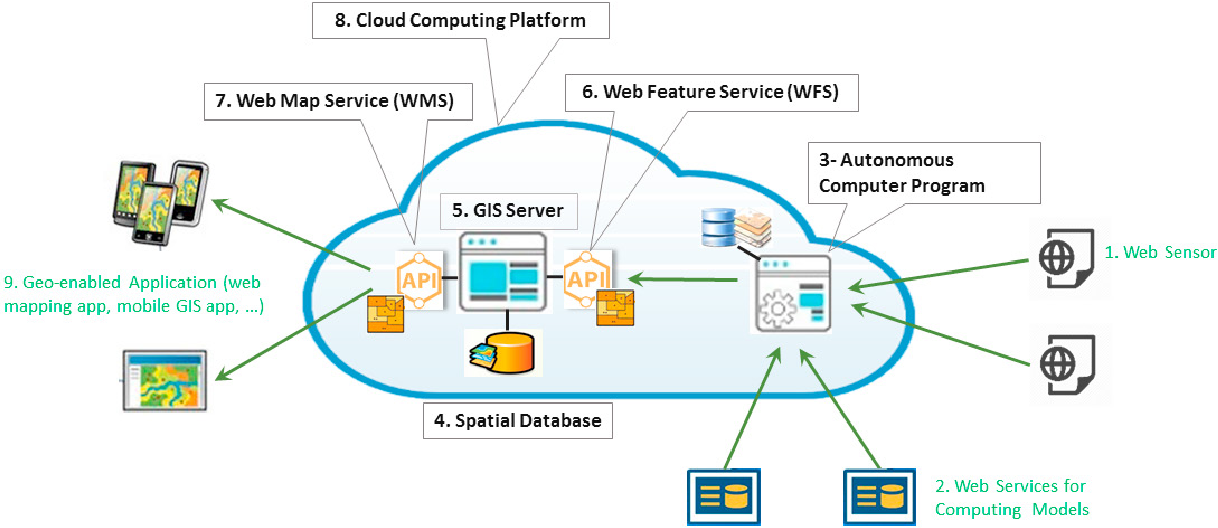
\includegraphics[width=0.8\textwidth]{Imagenes/GIS/arquitecturaGIS.png}
  \caption{Arquitectura web GIS basada en la nube.} \label{fig:arquitecturaGIS}
\end{figure}

En la figura \ref{fig:arquitecturaGIS} se muestra un esquema con los distintos componentes que forman la arquitectura de un GIS basado en la nube.
En concreto, vemos la infraestructura empleada para el despliegue de los servicios GIS y su interacción con los usuarios de tales servicios.
Los usuarios acceden en tiempo real a los servicios GIS a través de Internet por medio de un Servicio Web o API (puntos 1 y 2).
También el servicio puede ser consumido por una aplicación web (punto 3) para acceder a sus datos o funcionalidad. 
La propia plataforma (punto 8) contiene una aplicación web que se conecta al servidor GIS (punto 5) para recibir y recopilar datos geográficos. 
La aplicación permite manipular estos datos, es decir, permite realizar operaciones CRUD \textit{(Create, Read, Update, Delete)} con la base de datos espaciales (punto 4).
Los datos son el núcleo de cualquier GIS, por ello, la BBDD espacial debe mantener los datos disponibles y accesibles en todo momento.
Para ello, es necesario que permita el acceso a los datos en tiempo real, ya que los datos son capturados en tiempo real y se perdería la coherencia en determinadas aplicaciones.
La BBDD espacial también debe ser editable y replicable, para mantener la integridad de los datos.
Por último, en las arquitecturas GIS basadas en la nube, la BBDD espacial debe estar integrada en la infraestructura cloud en la que están el resto de servicios.

El servidor GIS expone la información a través de distintos estándares de servicios web (estándares OGC), servicios que cumplen con una serie de normas de intercambio de información desarrolladas por el Open Geospatial Consortium,
entre los cuales destacan el WMS, Servicio de Mapas Web (punto 7), y el WFS, Servicio de Objetos Espaciales (punto 6).
El protocolo WMS permite servir imágenes georeferenciadas a través de internet, es decir, permite obtener mapas y capas en formato imagen.
En cambio, el protocolo WFS permite realizar peticiones al servidor sobre elementos u objetos (features) geográficos individualizados,
de modo que podremos acceder no sólo a las geometrías de los elementos sino también a los atributos de los mismos.

\section{Herramientas}\label{sec:herramientas}

En los últimos años han aparecido en el mercado numerosas herramientas de desarrollo de GIS, que facilitan el desarrollo de aplicaciones SIG.
Estas herramientas se caracterizan por ofrecer a los desarrolladores las funcionalidades básicas para la gestión y almacenamiento de información,
junto con ciertas facilidades para el desarrollo de interfaces de captura y consulta de los datos.

Entre las herramientas que actualmente lideran el mercado del desarrollo GIS, destacan \textit{QGIS} y \textit{ArcGIS}.

\textit{QGIS} es el GIS líder de código abierto para escritorio, licenciado bajo GNU - General Public License y desarrollado por Open Source Geospatial Foundation (OSGeo), 
organización sin ánimo de lucro centrada en el ámbito de la tecnología geoespacial, con filosofía de software libre y desarrollo participativo.
Por ello, \textit{QGIS} cuenta con una gran comunidad que contribuye en forma de corrección de errores, implementación de plugins y en menor medida en aportaciones de documentación.

Por otro lado, \textit{ArcGIS} agrupa un conjunto de aplicaciones GIS de pago, comercializadas por \textit{ESRI} (Environmental Systems Research Institute), empresa norteamericana líder del sector.
A diferencia de \textit{QGIS}, presenta una documentación muy detallada y además, engloba una familia de aplicaciones online (\textit{ArcGIS Server}), permitiendo crear y compartir mapas web interactivos, lo que facilita el trabajo colaborativo con este tipo de información.

\textit{QGIS} resulta una opción más interesante cuando nos interesa trabajar con distintos sistemas operativos, ya se puede instalar en mac, linux o windows, 
en cambio \textit{ArcGIS} sólo se puede instalar en windows, según la especificación oficial de requisitos de instalación \cite{arcgis-instalation-requirements}.
\textit{QGIS} también permite disponer de un conjunto amplio de herramientas y plugins de forma gratuita, sin necesidad de licencia, debido a su condición de software libre.

\section{Aplicaciones}

Existen numerosas formas en las que los GIS son utilizados en la industria. Algunos ejemplos son:

\begin{itemize}
  \item Los equipos de respuesta a emergencias para definir movimientos en situaciones de desastres naturales.
  \item Las autoridades para descubrir cualquier humedal potencial que deba protegerse de los efectos nocivos provocados por la contaminación.
  \item Las empresas para elegir una ubicación de mercado estratégica que aún no haya sido saturada por otros competidores.
  \item El personal sanitario para predecir cualquier posible propagación de enfermedades y pandemias que siguen los mismos patrones de propagación.
\end{itemize}